\begin{frame}[label=IF_sucks]
    \frametitle{Challenges of Interferometry}
    \begin{columns}
        \begin{column}{0.7\textwidth}
            Requirements:
            \begin{itemize}
                \item \alert{Precise array positioning}
                \item Tedious \alert{calibration} of {every} link
                \item Periodic \alert{re-calibration}  
            \end{itemize}

            Other drawbacks: 
            \begin{itemize}
                \item Positional \alert{uncertainties are difficult} to estimate
                \item Performance drops off or fails low at SNRs, so these \alert{observations are discarded}
            \end{itemize}
            \centering
            \begin{tcolorbox}[width = 0.8\linewidth, center, boxrule=0pt,colback=yellow,arc=0pt,outer arc = 0pt,left=0pt,right=0pt,boxsep=2pt]
            \centering
            \textbf{Interferometry makes deployment, operation, and analysis difficult!}
        \end{tcolorbox}
        \end{column}
        \begin{column}{0.3\textwidth}
            \centering
            \begin{tikzpicture}
                \node[anchor=center, inner sep=0] (img) at (0,0) {
                    {{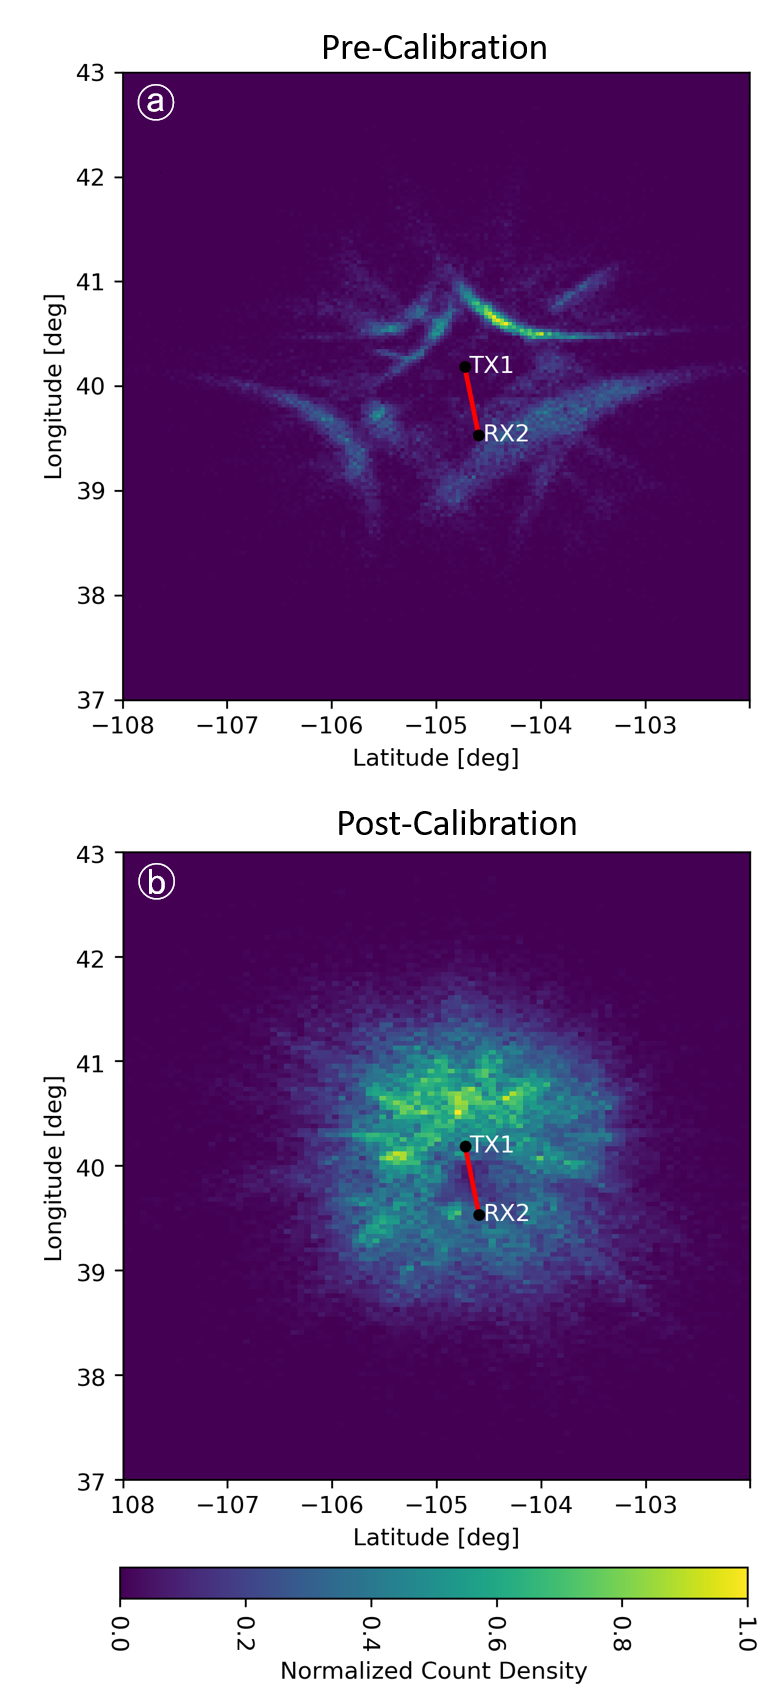
\includegraphics[height=\textheight - 1.5cm]{img/calibration_vert.png}}}
                };
                \node[anchor=north east, inner sep=2pt] at ([yshift=-0.3cm]img.north east) { 
                    {{{\fontsize{3}{3.4}\selectfont\raggedleft \textcolor{white}{\textit{Credit:} \citeauthor{marino_MeteorRadarPhase_2024}, \citeyear{marino_MeteorRadarPhase_2024} \cite{marino_MeteorRadarPhase_2024}}}}}
                };
            \end{tikzpicture}
        \end{column}
    \end{columns}
\end{frame}